
\section{Sistemi termici}
Al fine di descrivere i sistemi termici è fondamentale conoscere l'equazione
del bilancio termico.

Si considera un certo volume di superficie $S$ caratterizzato da un unico
parametro: la \textit{capacità termica}; la capacità termica di un corpo è
l'attitudine del corpo a modificare la sua temperatura quando questo viene
investito da una certa potenza termica.

È inoltre esprimibile come il rapporto tra il calore entrante nel corpo e la
variazione di temperatura che esso subisce, è considerata un'inerzia termica.
Il volume può interagire con l'ambiente che lo circonda mediante la superficie
$S$, quest'ultima consente di realizzare gli scambi di potenza termica.
%Posizione della figure non specificata, [h] missing
% è una prova dell'impaginamento automatico di LaTex
\begin{figure}
 \centering
 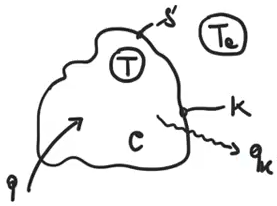
\includegraphics[width=\picwid]{corpo_termico.png}
 % corpo_termico.png: 277x206 px, 96dpi, 7.33x5.45 cm, bb=0 0 208 154
 \label{Fig.:corpo_termico}
\end{figure}

Si suppone inoltre che il corpo abbia una temperatura uniforme $T$, costante in
ogni suo punto, l'ambiente esterno invece sarà ad una temperatura $T_a\neq T$.

La differenza tra le due temperature genererà dei flussi di potenza termica dal
corpo (o ambiente) più caldo a quello più freddo.
La quantità di energia termica che attraversa la superficie dipenderà dalla
superficie stessa e in particolare dalla sua \textit{resistenza termica}.

Si indica con $K$ il coefficiente di scambio termico che la superficie consente
di sviluppare.
Il flusso termico $q_K$ è definito per convenzione positivo se uscente dal
corpo, dunque
$$
q_K = K(T-T_a)
$$

Si riportano le equazioni di bilancio termico che interessano il volume se
questo è sottoposto ad $n$ flussi termici $q_n$ ed $i$ superfici di scambio
termico con coefficiente di scambio $K_i$ e con ambienti a temperature $T_i$
(diverse o meno fra loro):
$$
C\dot{T} = \sum_n q_n -\sum_i K_i(T-T_i)
$$

Si riporta il modello ISU del sistema in esame con una sola potenza termica in
ingresso ed un solo scambio termico con un unico ambiente
 a temperatura $T_a$
$$
C\dot{T} = q -K(T-T_a)
$$
variabili:
$$\begin{matrix}
q & T_a & T \\
(0) & (0) & (1) \\
u_1 & u_2 & x
\end{matrix}
$$
\emph{Attenzione, $T_a$ è a tutti gli effetti una variabile di ingresso, anche
se resta costante, si parla di ingresso non manipolabile}

Equazioni del sistema:
$$\left\{\begin{aligned}
\dot{x} &=  \dot{T} = \frac{1}{C}u_1-K(x-u_2) \\
y &= T = x
\end{aligned}\right.$$

\subsection{Esempio forno elettrico}
Dato un volume chiuso si indica con $C_1$ la sua capacità termica e $T_1$ la
sua temperatura.
Si suppone che sia presente attorno al volume una parete con capacità termica
$C_2$ ed una temperatura supposta uniforme $T_2$, l'ambiente esterno è alla
temperatura $T_a$.
All'interno del volume è presente una resistenza elettrica che fornisce una
certa potenza termica $q$.

\begin{figure}[h]
 \centering
 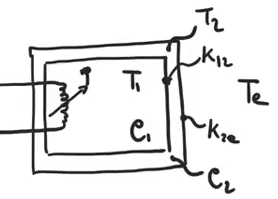
\includegraphics[width=\picwid]{forno_elettrico.png}
 % forno_elettrico.png: 278x199 px, 96dpi, 7.35x5.26 cm, bb=0 0 208 149
 \label{Fig.:forno_elettrico}
\end{figure}

Attraverso la parete, la temperatura è in realtà un gradiente termico e non
uniforme.
Si indicano con $K_{12}$ e $K_{2a}$ i coefficienti di scambio termico tra le
rispettive superfici.

Per ogni volume con una certa capacità termica, va scritta un'equazione del
bilancio
$$\left\{\begin{aligned}
C_1\dot T_1 &= q - K_{12}(T_1-T_2)\\
C_2\dot{T}_2 &= -K_{12}(T_2-T_1) - K_{2a}(T_2-T_a)
\end{aligned}\right.$$
Si nota come il flusso termico $K_{12}(T_1-T_2)$ uscente dal primo volume sia
entrante nel secondo.
Utilizzando sempre la stessa convenzione sui versi non si commettono errori e
non bisogna riflettere sui versi effettivo dei flussi termici.

Variabili:
$$\begin{matrix}
q & T_a & T_1 & T_2 \\
(0) & (0) & (1) & (1) \\
u_1 & u_2 & x_1 & x_2
\end{matrix}$$
Il sistema è di ordine due.

$$\left\{\begin{aligned}
\dot x_1 &= \dot{T}_1
\end{aligned}\right.$$
29:23
